

%%% Paper content

\chapter{
	\centering{Learn the Time to Learn: Replay Scheduling in Continual Learning}
}\label{chap:paperC}
\chaptermark{Replay Scheduling in Continual Learning}
\vspace{-5mm}
\begin{center}
	\large{\textbf{Marcus Klasson$^{*}$, Hedvig Kjellström$^{*}$, Cheng Zhang$^{\dagger}$}} \\[2mm]
	\small{$^{*}$KTH Royal Institute of Technology, Stockholm, Sweden} \\
	\small{$^{\dagger}$Microsoft Research, Cambridge, United Kingdom} \\
\end{center}


%%%%%%%%%%%%%%%%%%%%%%%%%%%%%%%%%%%%%%%%%%%%%%%%%%%%%%%%%%%%%%%%%%%%%%%%%%%%%%%%
%%%%%%%%%%%%%%%%%%%%%%%%%%%%%%%%%%%%%%%%%%%%%%%%%%%%%%%%%%%%%%%%%%%%%%%%%%%%%%%%
\begin{abstract}
	%\printinunitsof{in}\prntlen{\linewidth}
	\noindent Replay-based continual learning has shown to be successful in mitigating catastrophic forgetting, where most works focus on improving the sample quality in the commonly small replay memory. However, in many real-world applications, replay memories would be limited by constraints on processing time rather than storage capacity as most organizations store all historical data in the cloud. Inspired by human learning, we demonstrate that scheduling over the time to replay is critical to the final performance with finite memory resources. To this end, we propose to learn the time to learn for a continual learning system, in which we learn schedules over which tasks to replay at different times. We use Monte Carlo tree search to illustrate this idea and show that our method can be combined with any replay-based method and memory selection technique. We perform extensive evaluation showing that learning replay schedules can significantly improve the performance compared to baselines without learned scheduling. Our results indicate that the learned schedules are also consistent with human learning insights.
\end{abstract}


%%% Contents
%
\section{Introduction}\label{paperC:sec:introduction}

Many organizations deploying machine learning systems receive large volumes of data daily~\citeC{C:bailis2017macrobase, C:hazelwood2018applied}. Although all historical data are stored in the cloud in practice, retraining machine learning systems on a daily basis is prohibitive both in time and cost. In this setting, the systems often need to continuously adapt to new tasks while retaining the previously learned abilities. Continual learning (CL) methods~\citeC{C:delange2021continual, parisi2019continual} address this challenge where, in particular, replay methods~\citeC{C:chaudhry2019tiny, C:hayes2020remind} have shown to be very effective in achieving great prediction performance. 
Replay methods mitigate catastrophic forgetting by revisiting a small set of samples, which is feasible to process compared to the size of the historical data. In the traditional CL literature, replay memories are limited due to the assumption that historical data are not available. In the real-world setting where historical data are in fact always available, the requirement of small memory remains due to processing time and cost issues. 

%Many organizations deploying machine learning systems receive large volumes of data daily where these new data are often associated with new tasks. Although all historical data are stored in the cloud in practice, retraining machine learning systems on a daily basis is prohibitive both in time and cost. In this setting, the systems must continuously adapt to new tasks without forgetting the previously learned abilities. Continual learning (CL) methods~\citeC{C:de2019continual, C:parisi2019continual} address this challenge where, in particular, replay-based methods~\citeC{C:chaudhry2019tiny, C:hayes2020remind} have shown to be very effective in achieving great prediction performance and retaining knowledge of old tasks. Replay-based methods mitigate catastrophic forgetting by revisiting a small set of samples, which is feasible to process compared to the size of the historical data. In the traditional CL literature, the replay memory is limited due to the assumption that historical data are not available. In the real-world setting where historical data are in fact always available, the requirement of small memory remains due to processing time and cost issues. % 

Recent research on replay-based CL has focused on the quality of memory samples
~\citeC{C:aljundi2019gradient, C:borsos2020coresets, C:chaudhry2019tiny, C:chrysakis2020online, C:nguyen2017variational, C:rebuffi2017icarl, C:yoon2021online} 
or data compression to increase the memory capacity~\citeC{C:hayes2020remind, C:iscen2020memory, C:pellegrini2019latent}. 
Most previous methods allocate equal memory storage space for samples from old tasks, and replay the whole memory to mitigate catastrophic forgetting.
However, in life-long learning settings, this simple strategy would be inefficient as the memory must store a large number of tasks.
Furthermore, uniform selection policy of samples to revisit is commonly used which ignores the time of which tasks to learn again. This stands in contrast to human learning where education methods focus on scheduling of learning and rehearsal of previous learned knowledge. For example, spaced repetition~\citeC{dempster1989spacing, ebbinghaus2013memory, landauer1978optimum}, where the time interval between rehearsal increases, has been shown to enhance memory retention. 

%Most research on replay-based CL has been focused on the sample quality in the memory~\citeC{C:aljundi2019gradient, C:borsos2020coresets, C:chaudhry2019tiny, C:chrysakis2020online, C:nguyen2017variational, C:rebuffi2017icarl, C:yoon2021online} or data compression to increase the memory capacity~\citeC{C:hayes2020remind, C:iscen2020memory, C:pellegrini2019latent}. Common for these methods is that the memory allocates an equal amount of space for storing samples from old tasks. When learning new tasks, the whole memory is replayed to mitigate catastrophic forgetting. However, in life-long learning settings, this simple strategy would be inefficient as the memory must store a large number of tasks. Furthermore, these methods ignore the time to learn old tasks again which is important in human learning. Humans are CL systems, and different methods have been developed to enhance memory retention, such as spaced repetition~\citeC{C:dempster1989spacing, C:ebbinghaus2013memory, C:landauer1978optimum} which is often used in education. These education methods focus on the scheduling of learning and rehearsal of previous learned knowledge.  

\begin{figure}[t]
\centering
\setlength{\figwidth}{.25\textwidth}
\setlength{\figheight}{.15\textheight}
% This file was created by tikzplotlib v0.9.8.
\pgfplotsset{every axis title/.append style={at={(0.5,0.83)}}}
\pgfplotsset{every axis x label/.append style={at={(0.5,-0.30)}}}
\pgfplotsset{every major tick/.append style={major tick length=2pt}}
\pgfplotsset{every minor tick/.append style={minor tick length=1pt}}
\pgfplotsset{every tick label/.append style={font=\scriptsize}}
\begin{tikzpicture}
\tikzstyle{every node}=[font=\scriptsize]
\definecolor{color0}{rgb}{0.12156862745098,0.466666666666667,0.705882352941177}
\definecolor{color1}{rgb}{1,0.498039215686275,0.0549019607843137}
\definecolor{color2}{rgb}{0.172549019607843,0.627450980392157,0.172549019607843}
\definecolor{color3}{rgb}{0.83921568627451,0.152941176470588,0.156862745098039}
\definecolor{color4}{rgb}{0.580392156862745,0.403921568627451,0.741176470588235}

\begin{groupplot}[group style={group size=4 by 1, horizontal sep=1.0cm,}]
\nextgroupplot[title={ACC: 89.66\%},
legend cell align={left},
%legend columns=-1,
%legend style={
%  nodes={scale=0.9},
%  fill opacity=0.8,
%  draw opacity=1,
%  text opacity=1,
%  at={(0.03,1.27)},
%  anchor=south west,
%  draw=white!80!black
%},
height=\figheight,
minor xtick={},
minor ytick={0.65,0.75,0.85,0.95,1,1.1},
tick align=outside,
tick pos=left,
width=\figwidth,
x grid style={white!69.0196078431373!black},
xlabel={Task},
xmajorgrids,
xmin=0.8, xmax=5.2,
xtick style={color=black},
xtick={1,2,3,4,5},
xticklabels={1,2,3,4,5},
y grid style={white!69.0196078431373!black},
ylabel={Accuracy(\%)},
ymajorgrids,
yminorgrids,
ymin=0.7, ymax=1.01,
ytick style={color=black},
ytick={0.6,0.7,0.8,0.9,1,1.1},
yticklabels={60,70,80,90,100,110}
]
\addplot [line width=1.5pt, color0, mark=*, mark size=1, mark options={solid}]
table {%
1 0.999527156352997
2 0.997730553150177
3 0.882458686828613
4 0.794799029827118
5 0.841323971748352
};
%\addlegendentry{Task 1}
\addplot [line width=1.5pt, color1, mark=*, mark size=1, mark options={solid}]
table {%
2 0.995984375476837
3 0.963858962059021
4 0.868658185005188
5 0.76601368188858
};
%\addlegendentry{Task 2}
\addplot [line width=1.5pt, color2, mark=*, mark size=1, mark options={solid}]
table {%
3 0.998612582683563
4 0.950907111167908
5 0.886979699134827
};
%\addlegendentry{Task 3}
\addplot [line width=1.5pt, color3, mark=*, mark size=1, mark options={solid}]
table {%
4 0.999194324016571
5 0.993353486061096
};
%\addlegendentry{Task 4}
\addplot [line width=1.5pt, color4, mark=*, mark size=1, mark options={solid}]
table {%
5 0.995259761810303
};
%\addlegendentry{Task 5}
\addplot [line width=1.5pt, black, dashed]
table {%
2 0
2 1.05
};
%\addlegendentry{Replay}

\nextgroupplot[title={ACC: 93.85\%},
height=\figheight,
minor xtick={},
minor ytick={0.65,0.75,0.85,0.95,1,1.1},
tick align=outside,
tick pos=left,
width=\figwidth,
x grid style={white!69.0196078431373!black},
xlabel={Task},
xmajorgrids,
xmin=0.8, xmax=5.2,
xtick style={color=black},
xtick={1,2,3,4,5},
xticklabels={1,2,3,4,5},
y grid style={white!69.0196078431373!black},
%ylabel={Accuracy},
ymajorgrids,
yminorgrids,
ymin=0.7, ymax=1.01,
ytick style={color=black},
ytick={0.6,0.7,0.8,0.9,1,1.1},
yticklabels={60,70,80,90,100,110}
]
\addplot [line width=1.5pt, color0, mark=*, mark size=1, mark options={solid}]
table {%
1 0.999527156352997
2 0.990638375282288
3 0.998770713806152
4 0.954420864582062
5 0.953191578388214
};
%\addlegendentry{Task 1}
\addplot [line width=1.5pt, color1, mark=*, mark size=1, mark options={solid}]
table {%
2 0.995102763175964
3 0.970029354095459
4 0.915377020835876
5 0.799706101417542
};
%\addlegendentry{Task 2}
\addplot [line width=1.5pt, color2, mark=*, mark size=1, mark options={solid}]
table {%
3 0.998505890369415
4 0.964674472808838
5 0.954108893871307
};
%\addlegendentry{Task 3}
\addplot [line width=1.5pt, color3, mark=*, mark size=1, mark options={solid}]
table {%
4 0.999395728111267
5 0.990936577320099
};
%\addlegendentry{Task 4}
\addplot [line width=1.5pt, color4, mark=*, mark size=1, mark options={solid}]
table {%
5 0.994755387306213
};
%\addlegendentry{Task 5}
\addplot [line width=1.5pt, black, dashed]
table ,
height=\figheight,
minor xtick={},
minor ytick={0.65,0.75,0.85,0.95,1,1.1},
tick align=outside,
tick pos=left,
width=\figwidth,
x grid style={white!69.0196078431373!black},
xlabel={Task},
xmajorgrids,
xmin=0.8, xmax=5.2,
xtick style={color=black},
xtick={1,2,3,4,5},
xticklabels={1,2,3,4,5},
y grid style={white!69.0196078431373!black},
%ylabel={Accuracy},
ymajorgrids,
yminorgrids,
ymin=0.7, ymax=1.01,
ytick style={color=black},
ytick={0.6,0.7,0.8,0.9,1,1.1},
yticklabels={60,70,80,90,100,110}
]
\addplot [line width=1.5pt, color0, mark=*, mark size=1, mark options={solid}]
table {%
1 0.999527156352997
2 0.990638375282288
3 0.784302592277527
4 0.994799017906189
5 0.979763627052307
};
%\addlegendentry{Task 1}
\addplot [line width=1.5pt, color1, mark=*, mark size=1, mark options={solid}]
table {%
2 0.995102763175964
3 0.967384934425354
4 0.902546525001526
5 0.736434817314148
};
%\addlegendentry{Task 2}
\addplot [line width=1.5pt, color2, mark=*, mark size=1, mark options={solid}]
table {%
3 0.998185753822327
4 0.962860226631165
5 0.960298895835876
};
%\addlegendentry{Task 3}
\addplot [line width=1.5pt, color3, mark=*, mark size=1, mark options={solid}]
table {%
4 0.998892307281494
5 0.988116860389709
};
%\addlegendentry{Task 4}
\addplot [line width=1.5pt, color4, mark=*, mark size=1, mark options={solid}]
table {%
5 0.994049429893494
};
%\addlegendentry{Task 5}
\addplot [line width=1.5pt, black, dashed]
table ,
height=\figheight,
legend columns=1,
legend style={
  nodes={scale=0.75},
  fill opacity=0.8,
  draw opacity=1,
  text opacity=1,
  at={(1.13,-0.3)},
  anchor=south west,
  draw=white!80!black
},
minor xtick={},
minor ytick={0.65,0.75,0.85,0.95,1,1.1},
tick align=outside,
tick pos=left,
width=\figwidth,
x grid style={white!69.0196078431373!black},
xlabel={Task},
xmajorgrids,
xmin=0.8, xmax=5.2,
xtick style={color=black},
xtick={1,2,3,4,5},
xticklabels={1,2,3,4,5},
y grid style={white!69.0196078431373!black},
%ylabel={Accuracy},
ymajorgrids,
yminorgrids,
ymin=0.7, ymax=1.01,
ytick style={color=black},
ytick={0.6,0.7,0.8,0.9,1,1.1},
yticklabels={60,70,80,90,100,110}
]
\addplot [line width=1.5pt, color0, mark=*, mark size=1, mark options={solid}]
table {%
1 0.999527156352997
2 0.990638375282288
3 0.784302592277527
4 0.645106375217438
5 0.995650112628937
};
\addlegendentry{Task 1}
\addplot [line width=1.5pt, color1, mark=*, mark size=1, mark options={solid}]
table {%
2 0.995102763175964
3 0.967384934425354
4 0.905876517295837
5 0.780019640922546
};
\addlegendentry{Task 2}
\addplot [line width=1.5pt, color2, mark=*, mark size=1, mark options={solid}]
table {%
3 0.998185753822327
4 0.969583809375763
5 0.966808974742889
};
\addlegendentry{Task 3}
\addplot [line width=1.5pt, color3, mark=*, mark size=1, mark options={solid}]
table {%
4 0.999295055866241
5 0.987814724445343
};
\addlegendentry{Task 4}
\addplot [line width=1.5pt, color4, mark=*, mark size=1, mark options={solid}]
table {%
5 0.994452834129333
};
\addlegendentry{Task 5}
\addplot [line width=1.5pt, black, dashed]
table {%
5 0
5 1.05
};
\addlegendentry{Replay}
\end{groupplot}

\end{tikzpicture}

\vspace{-3mm}
\caption{Task accuracies on Split MNIST~\cite{C:zenke2017continual} when replaying only 10 samples of classes $0/1$ at a single time step. The black vertical line indicates when replay is used. ACC denotes the average accuracy over all tasks after learning Task 5. Results are averaged over 5 seeds. These results show that the time to replay the previous task is critical for the final performance.}
%This shows the time to learn the previous task again with memory is critical for the performance.
%}%\vspace{-4mm}
\label{fig:single_task_replay_with_M10}
\vspace{-2mm}
\end{figure}

We 
%In this work, we 
argue that finding the proper schedule of which tasks to replay in the fixed memory setting is critical for CL. To demonstrate our claim, we perform a simple experiment on the Split MNIST~\citeC{C:zenke2017continual} dataset where each task consists of learning the digits 0/1, 2/3, etc.\ arriving in sequence.
The replay memory contains data from task 1 and can only be replayed at one point in time.
Figure \ref{fig:single_task_replay_with_M10} shows how the task performances progress over time when the memory is replayed at different time steps. In this example, the best final performance is achieved when the memory is used when learning task 5.
Note that choosing different time points to replay the same memory leads to noticeably different results in the final performance. 
These results indicate that scheduling the time when to apply replay can influence the final performance significantly of a CL system.  

To this end, we propose learning the time to learn, in which we learn replay schedules of which tasks to replay at different times inspired from human learning~\citeC{C:dempster1989spacing}. 
To show the importance of replay scheduling, we take an episodic-learning approach where a policy is learned from multiple trials selecting which tasks to replay in a CL scenario. 
In particular, we illustrate in single CL environments by using Monte Carlo tree search (MCTS)~\citeC{C:coulom2006efficient} as an example method that searches for good replay schedules. %policies for replay. 
The replay schedules from MCTS are evaluated by measuring the final performance of a network trained on a sequence of CL tasks where the scheduled replay samples have been used for mitigating catastrophic forgetting. 
We use this way to show the importance of replay scheduling given an ideal environment to highlight the need for learning replay schedules in real-world large scale CL tasks. 
In summary, our contributions are:
\begin{itemize}[topsep=1pt,] %noitemsep,]
	\setlength\itemsep{0.1mm}
	\item We propose a new CL setting where historical data is available while the processing time is limited, in order to adjust current CL research closer to real-world needs (Section \ref{paperC:sec:problem_setting}). In this new setting, we introduce replay scheduling where we learn the time of which tasks to replay (Section \ref{paperC:sec:replay_scheduling_in_continual_learning}).

	\item We argue that learning the time to learn is essential for CL performance. We use MCTS as an example method to illustrate the benefits of replay scheduling in CL, where MCTS searches over finite sets of replay memory compositions at every task (Section \ref{paperC:sec:mcts_for_replay_scheduling}). 

	\item We demonstrate with six benchmark datasets that learned scheduling can improve the CL performance significantly in the fixed size memory setting (Section \ref{paperC:sec:results_with_mcts} and \ref{paperC:sec:results_with_varying_replay_memory_size}). 
	Moreover, we show that replay scheduling %our method 
	can be combined with any memory selection technique and replay-based method (Section \ref{paperC:sec:alternative_memory_selection_methods} and \ref{paperC:sec:applying_scheduling_to_recent_replay_methods}), as well as being efficient in situations where the 
	memory size is %even 
	smaller than the number of classes (Section \ref{paperC:sec:efficiency_of_replay_scheduling}). 
\end{itemize}






%
\section{Related Work}\label{paperC:sec:related_work}
In this section, we give a brief overview of CL methods, essentially replay-based methods, as well as spaced repetition techniques for human CL.

\vspace{-3mm}
\paragraph{Continual Learning.} Traditional CL can be divided into three main areas, namely regularization-based, architecture-based, and replay-based approaches. Regularization-based methods aim to mitigate catastrophic forgetting by protecting parameters influencing the predictive performance on known tasks from wide changes and use the rest of the parameters for learning new tasks~\citeC{C:adel2019continual, C:chaudhry2018riemannian, C:kirkpatrick2017overcoming, C:li2017learning, C:nguyen2017variational, C:rannen2017encoder, C:schwarz2018progress, zenke2017continual}. Architecture-based methods isolate task-specific parameters by either increasing network capacity~\citeC{C:rusu2016progressive, C:yoon2019scalable, C:yoon2017lifelong} or freezing parts of the network~\citeC{C:mallya2018packnet, C:serra2018overcoming} to maintain good performance on previous tasks. 
Replay-based methods mix samples from old tasks with the current dataset to mitigate catastrophic forgetting, where the replay samples are either stored in an external memory~\citeC{C:chaudhry2019tiny, C:hayes2020remind, C:isele2018selective, C:lopez2017gradient} or generated using a generative model~\citeC{C:shin2017continual, C:van2018generative}. 
%Replay-based methods store examples from previous tasks in an external memory~\citep{chaudhry2019tiny, hayes2020remind, isele2018selective, lopez2017gradient}, or uses a generative model to generate pseudo-samples from a distribution over tasks~\citep{shin2017continual, van2018generative}, that are mixed with the current task dataset to mitigate catastrophic forgetting. 
Regularization-based approaches and dynamic architectures have been combined with replay-based approaches to methods to overcome their limitations~\citeC{C:buzzega2020dark, C:chaudhry2018riemannian, C:chaudhry2018efficient, C:chaudhry2021using, C:douillard2020podnet, C:ebrahimi2020adversarial, C:joseph2020meta, C:mirzadeh2020linear, C:nguyen2017variational, C:pan2020continual, C:pellegrini2019latent, C:rolnick2018experience, C:von2019continual}. Our work relates most to replay-based methods with external memory which we spend more time on describing in the next paragraph.



\vspace{-3mm}
\paragraph{Replay-based Continual Learning.} A commonly used memory selection strategy of replay samples is random selection. 
%The simplest selection strategy is random selection of examples to store in the memory for replay. 
Much research effort has focused on selecting higher quality samples to store in memory~\citeC{C:aljundi2019gradient, C:borsos2020coresets, C:chaudhry2019tiny, C:chrysakis2020online, C:hayes2019memory, C:isele2018selective, C:lopez2017gradient, C:nguyen2017variational, C:rebuffi2017icarl, C:yoon2021online}. Chaudhry \etal~\citeC{C:chaudhry2019tiny} reviews several selection strategies in scenarios with tiny memory capacity, e.g., reservoir sampling~\citeC{C:vitter1985random}, first-in first-out buffer~\citeC{C:lopez2017gradient}, k-Means, and Mean-of-Features~\citeC{C:rebuffi2017icarl}. However, more elaborate selection strategies have been shown to give little benefit over random selection for image classification problems~\citeC{C:chaudhry2018riemannian, C:hayes2020remind}. More recently, there has been work on compressing raw images to feature representations to increase the number of memory examples for replay~\citeC{C:hayes2020remind, C:iscen2020memory, C:pellegrini2019latent}. 
Our approach differs from the above mentioned works since we focus on learning to select which tasks to replay at the current task rather than improving memory selection or compression quality of the memory samples. %samples in the memory. 
%Our approach differs from the above mentioned works since we focus on which memory examples to choose for training at the current task rather than which examples to store in the memory. 
Replay scheduling can however be combined with any selection strategy and feature compression method. %as well as storing features. %feature representations. 

%\CZ{Then start with the tradtionion random memory (your last two sentence. And then say what research has been focused on. E.g. Selection higher quility samples. e.g. VCL, Chauhry etc. Memory representations to store more data etc..... Then in the end say, we are focusing the scheduling and focus on learning when to learn. } Research has focused on various selection strategies, e.g. reservoir sampling and online k-means, for which samples to store in memory~\citep{chaudhry2019tiny, hayes2019memory, rebuffi2017icarl}. Chaudhry \etal~\citep{chaudhry2019tiny} reviews several selection strategies \CZ{What are these trategies?} in scenarios with tiny memory capacity, and Hayes\etal~\citep{hayes2019memory} develops a strategy based on online k-means. However, most commonly the replay samples are selected uniformly at random depending on the experimental setting. Another line of work focuses on increasing the memory capacity by storing past examples a feature representations instead of raw format~\citep{hayes2020remind}. 

%Another important aspect of memory-based methods is how to adjust the memory size when storing old examples from the most recent task. There exist two popular approaches for setting the memory size that maintain an equal distribution of past examples in the memory, which is important when the memory size is small. In the first strategy, a constant number of samples per class $M_{per}$ are stored, so that the total memory size grows with the number of classes~\citep{douillard2020podnet, hou2019learning}. The second strategy sets a fixed size capacity on the memory meaning that we are only allowed to store a total of $M_{total}$ number of samples from all previously seen classes/tasks~\citep{chaudhry2019tiny, lopez2017gradient}. For our task, we assume that we can easily access historical data and focus on which tasks to select for replay. In Section \ref{sec:replay_scheduling_for_continual_learning}, we describe our memory setting for learning policies to select replay schedules.


\vspace{-3mm}
\paragraph{Human Continual Learning.} Humans are CL systems in the sense of learning tasks and concepts sequentially. Furthermore, humans have the ability to memorize experiences but forgets learned knowledge gradually rather than catastrophically~\citeC{C:french1999catastrophic}. Different learning techniques have been suggested for humans to memorize better~\citeC{C:dunlovsky2013improving, C:willis2007review}. 
An example is spaced repetition where time intervals between rehearsal are gradually increased to improve long-term memory retention~\citeC{C:dempster1989spacing}, where the earliest documented works are from Ebbinghaus~\citeC{C:ebbinghaus2013memory}. %An example is spaced repetition which gradually increases time-intervals between rehearsals for retaining long-term memory~\citep{dempster1989spacing}, where the earliest documented works are from \citet{ebbinghaus2013memory}. 
Further studies have shown that memory training schedules with adjusted spaced repetition are better at preserving memory than using uniformly spaced rehearsal times~\citeC{C:hawley2008comparison, C:landauer1978optimum}. 
%An example is spaced repetition which gradually increases time-intervals between rehearsals for retaining long-term memory~\citep{dempster1989spacing}. 
%This technique has been studied frequently and was inspired from the works of \citet{ebbinghaus2013memory} on memory retention. 
%For example, \citet{landauer1978optimum} demonstrated that memory training schedules using adjusted spaced repetition were better at preserving memory than uniformly spaced training. 
%\citet{hawley2008comparison} studies the efficacy of spaced repetition on adults with probable Alzheimer's disease for learning face-name association.  
Several works in CL with neural networks are inspired by %or have connections to 
human learning techniques, including spaced repetition~\citeC{C:amiri2017repeat, C:feng2019spaced, C:smolen2016right}, %~\citep{amiri2017repeat, amiri2019neural, feng2019spaced, smolen2016right}, 
sleep mechanisms~\citeC{C:ball2020study, C:mallya2018packnet, C:schwarz2018progress}, %mechanisms of sleep~\citep{ball2020study, mallya2018packnet, schwarz2018progress}, 
and memory reactivation~\citeC{C:hayes2020remind, C:van2020brain}. % reactivation of memories~\citep{hayes2020remind, van2020brain}. 
Replay scheduling is also inspired by spaced repetition, where %Our replay scheduling method is inspired by spaced repetition; %where 
we learn schedules of which tasks to replay at different times. % steps. %memory samples to use for replay at different time steps. 


%\section{Our Dataset}\label{paperA:sec:our-dataset}

We have collected images from fruit and vegetable sections and refrigerated sections with dairy and juice products in 18 different grocery stores. The dataset consists of 5125 images from 81 fine-grained classes, where the number of images in each class range from 30 to 138. Figure \ref{fig:hist} displays a histogram over the number of images per class. As illustrated in Figure \ref{fig:examples}, the class structure is hierarchical, and there are 46 coarse-grained classes. Figure \ref{fig:dataset-figure} shows examples of the collected natural images. For each fine-grained class, we have downloaded an iconic image of the item and also a product description including origin country, an appreciated weight and nutrient values of the item from a grocery store website. Some examples of downloaded iconic images can be seen in Figure \ref{fig:clean-image-figure}. 

Our aim has been to collect the natural images under the same condition as they would be as part of an assistive application on a mobile phone. All images have been taken with a 16-megapixel Android smartphone camera from different distances and angles. Occasionally, the images include other items in the background or even items that have been misplaced in the wrong shelf along with the targeted item. It is important that image classifiers that are used for assisting devices are capable of performing well with such noise since these are typical settings in a grocery store environments. The lighting conditions in the images can also vary depending on where the items are located in the store. 
Sometimes the images are taken while the photographer is holding the item in the hand. This is often the case for refrigerated products since these containers are usually stacked compactly in the refrigerators. For these images, we have consciously varied the position of the object, such that the item is not always centered in the image or present in its entirety. 

We also split the data into a training set and test set based on the application need. Since the images have been taken in several different stores at specific days and time stamps, 
parts of the data will have similar lighting conditions and backgrounds for each photo occasion. To remove any such biasing correlations, all images of a certain class taken at a certain store are assigned to either the test set or training set. Moreover, we balance the class sizes to as large extent as possible in both the training and test set. After the partitioning, the training and test set contains 2640 and 2485 images respectively. Predefining a training and test set also makes it easier for other users to compare their results to the evaluations in this paper.

The task is to classify natural images using mobile devices to aid visually impaired people. The additional information such as the hierarchical structure of the class labels, iconic images, and product descriptions can be used to improve the performance of the computer vision system. Every class label is associated with a product description. Thus, the product description itself can be part of the output for visually impaired persons as they may not be able to read what is printed on a carton box or a label tag on a fruit bin in the store.

%Collecting and labeling real-world data is a time-costly procedure. 
%Therefore, we propose that the natural images can be combined with additional information of the target object in the form of text and iconic images.
The dataset is intended for research purposes and we are open to contributions with more images and new suitable classes. Our dataset is available at \url{https://github.com/marcusklasson/GroceryStoreDataset}. Detailed instructions on how to contribute to the dataset can be found on our dataset webpage.



\begin{figure}[t]
\centering
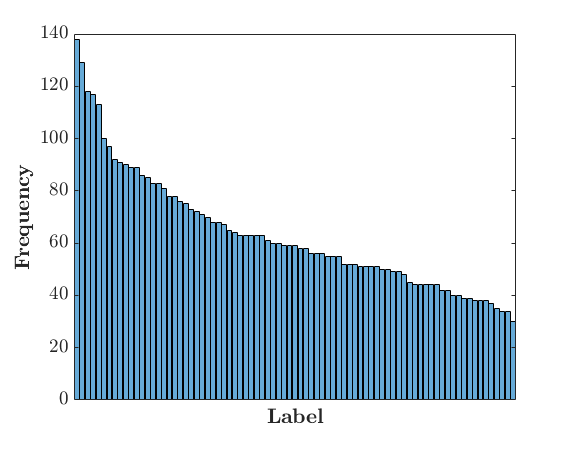
\includegraphics[width=\columnwidth,height=0.20\paperheight]{PaperA/figures/hist1_latex_bf14.png}
\caption{Histogram over the number of images in each class in the dataset.}
\label{fig:hist}
\end{figure}


%\section{Experimental Results}\label{sec:experimental-results}

We apply the three different types of models described in Section \ref{sec:classification-methods} to our dataset and evaluate their performance. The natural images are propagated through a CNN pretrained on ImageNet to extract feature vectors. We experiment with both the off-the-shelf features as well as fine-tuning the CNN. When using off-the-shelf features, we simply extract feature vectors and train an SVM on those. For the fine-tuned CNN, we report both results from the softmax classifier used in the actual fine-tuning procedure and training an SVM with extracted fine-tuned feature vectors.  

These extracted feature vectors are also used for VAE and VAE-CCA which makes further compression. We perform classification for those VAE based models by training a classifier, e.g. an SVM, on the data encoded into the latent representation. We use this classification approach for both VAE and VAE-CCA. In all classification experiments, except when we fine-tune the CNN, we use a linear SVM trained with the one-vs-one approach as in \cite{razavian2014cnnfeatures}.

We experiment with three different pretrained CNN architectures, namely AlexNet \cite{krizhevsky2012imagenet}, VGG16 \cite{simonyan2014verydeep} and DenseNet-169 \cite{huang2017densely}. For AlexNet and VGG16, we extract feature vectors of size 4096 from the two last fully connected (FC) layers before the classification layer. The features from the $n^{\text{th}}$ hidden layer are denoted as $\text{AlexNet}_{n}$ and $\text{VGG16}_{n}$. As an example, the last hidden FC layer in AlexNet is denoted as $\text{AlexNet}_{7}$, the input of which is output from $\text{AlexNet}_{6}$. For DenseNet-169, we extract the features of size 1664 from the average pooling layer before its classification layer.

\renewcommand{\arraystretch}{1.2}
\begin{table*}[t]
    \centering
    \caption{ Fine-grained classification (81 classes) accuracies with the methods described in Section \ref{subsec:experimental-setups}. Each row displays from which network architecture and layer that we extracted the feature vectors of the natural images. The columns show the result from the classifiers that we used (see Section \ref{subsec:experimental-setups}). }
    \vspace{2mm}
    \begin{tabular}{c | c c | c c | c c}
        \hline
        \Xhline{3\arrayrulewidth}
        & SVM & SVM-ft & VAE+SVM & VAE+SVM-ft & VAE-CCA+SVM & VAE-CCA+SVM-ft  \\
        \Xhline{3\arrayrulewidth}
        \rowcolor{Gray}
         $\text{AlexNet}_{6}$  &  69.2 & 72.6 & 65.6 & 70.7 & 67.8	& 71.5 \\
         $\text{AlexNet}_{7}$ &  65.0 & 70.7 & 63.0 & 68.7 & 65.0 & 70.9 \\
        \rowcolor{Gray}
         $\text{VGG16}_{6}$ &  62.1	& 73.3 & 57.5 & 71.9 & 60.7 & 73.0 \\
         $\text{VGG16}_{7}$ & 57.3	& 71.7 & 56.8 & 67.8 & 56.8 & 71.3 \\
        \rowcolor{Gray}
         $\text{DenseNet-169}$ & 72.5 & 85.0 & 65.4 & 79.1 & 72.6 & 80.4 \\
        \Xhline{3\arrayrulewidth}
    \end{tabular}
    \label{tab:results-fine-grained}
\end{table*}

\renewcommand{\arraystretch}{1.2}
\begin{table}[t]
    \centering
    \caption{Coarse-grained classification (46 classes) accuracies with an SVM for the methods described in Section \ref{subsec:experimental-setups} that uses off-the-shelf feature representations. Each row displays from network architecture and layer that we extracted the feature vectors of the natural images and the columns show the result for the classification methods. }
    \vspace{2mm}
    \scalebox{0.95}{
    \begin{tabular}{c | ccc}
        \Xhline{3\arrayrulewidth}
         & SVM & VAE+SVM & VAE-CCA+SVM  \\
        \Xhline{3\arrayrulewidth}
        \rowcolor{Gray}
         $\text{AlexNet}_{6}$ & 78.0 & 74.2 & 76.4  \\ 
         $\text{AlexNet}_{7}$ & 75.4 & 73.2 & 74.4  \\ 
        \rowcolor{Gray}
         $\text{VGG16}_{6}$ &  76.6 & 74.2 & 74.9  \\ 
         $\text{VGG16}_{7}$ & 72.8 & 71.7 & 72.3  \\
         \rowcolor{Gray}
         $\text{DenseNet-169}$ & 85.2 & 79.5 & 82.0 \\
        \Xhline{3\arrayrulewidth}
    \end{tabular}
    }
    \label{tab:results-coarse-grained}
\end{table}

\renewcommand{\arraystretch}{1.25}
\begin{table}[t]
\centering
\caption{Fine-grained classification accuracies from fine-tuned CNNs pretrained on ImageNet, where the column shows which architecture that has been fine-tuned. A standard softmax layer is used as the last classification layer.
}
\vspace{2mm}
\scalebox{0.95}{
\begin{tabular}{cccc}
    \hline
    \Xhline{3\arrayrulewidth}
    & AlexNet & VGG16 & DenseNet-169 \\
    \Xhline{3\arrayrulewidth}
    \rowcolor{Gray}
    Fine-tune &  69.3 & 73.8 & 84.0  \\
    \Xhline{3\arrayrulewidth}
\end{tabular}
}
\label{tab:results-finetuned-cnn}
\end{table}


\subsection{Experimental Setups}\label{subsec:experimental-setups}

The following setups were used in the experiments: 


\paragraph*{Setup 1.} Train an SVM on extracted off-the-shelf features from a pretrained CNN, which is denoted as SVM in the results. We also fine-tune the CNN by replacing the final layer with a new softmax layer and denote these results as Fine-tune. We denote training an SVM on extracted finetuned feature vectors as SVM-ft.


\paragraph*{Setup 2.} Extract feature vectors with a pretrained CNN of the natural images and learn a latent representation $\mathbf{z}$ with a VAE. Then the data is encoded into the latent space and we train an SVM with these latent representations, which used for classification. We denote the results as VAE+SVM when using off-the-shelf feature vectors, whereas using the fine-tuned feature vectors are denoted as VAE+SVM-ft. In all experiments with the VAE, we used the architecture from \cite{sohn2015conditionalvae}, i.e. the latent layer having 200 hidden units and both encoder and decoder consisting of two FC layers with 1,000 hidden units each.

\paragraph*{Setup 3.} Each natural image is paired with its corresponding iconic image. We train VAE-CCA similarly as the VAE, but instead, we learn a joint latent representation that is used to reconstruct the extracted feature vectors $\mathbf{x}$ and the iconic images $\mathbf{y}$. The classification is performed with the same steps as in Setup 2 and denotes the results similarly with VAE-CCA+SVM and VAE-CCA+SVM-ft. Our VAE-CCA model takes the feature vectors $\mathbf{x}$ as input and encodes them into a latent layer with 200 hidden units. The encoder and the feature vector decoder uses the same architecture, i.e. two FC layers with 512 hidden units, whereas the iconic image decoder uses the DCGAN \cite{radford2015unsupervised} architecture.

Figure \ref{fig:classification-methods} displays the three experimental setups described above. We report both fine-grained and coarse-grained classification results with an SVM in Table \ref{tab:results-fine-grained} and \ref{tab:results-coarse-grained} respectively. In Table \ref{tab:results-finetuned-cnn}, we report the fine-grained classification results from fine-tuned CNNs.

When fine-tuning the CNNs,
we replace the final layer with a softmax layer applicable to our dataset with randomly initialized weights drawn from a Gaussian with zero mean and standard deviation $0.01$~\cite{Zhang2014PartbasedRCNN}. 
For AlexNet and VGG16, we fine-tune the networks for 30 epochs with two different learning rates, 0.01 for the new classification layer and 0.001 for the pretrained layers. Both learning rates are reduced by half after every fifth epoch. The DenseNet-169 is fine-tuned for 30 epochs with momentum of $0.9$ and an initial learning rate of 0.001, which decays with $10^{-6}$ after each epoch. We report the classification results from the softmax activation after the fine-tuned classification layer. 
We also report classification results from an SVM trained with feature representations from a fine-tuned CNN, which are extracted from FC6 and FC7 of the AlexNet and VGG16 and from the last average pooling layer in DenseNet-169.

The VAE and VAE-CCA models are trained for 50 epochs with Adam \cite{kingma2015adam} for optimizing the ELBOs in Equation \ref{eq:vae-loss} and \ref{eq:vcca-loss} respectively. We use a constant learning rate of 0.0001 and set the minibatch size to 64. The extracted feature vectors are rescaled with standardization before training the VAE and VAE-CCA models to stabilize the learning.

\subsection{Results}
\begin{figure*}[t]
\centering
\subfigure[Royal Gala]{\label{subfig:royal-gala-natural}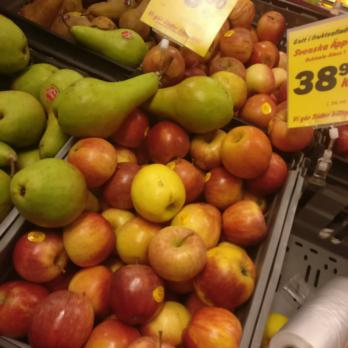
\includegraphics[width=0.33\columnwidth]{decoded-image-figure/Royal-Gala-Apple_003.jpg}}~
\subfigure[Decoded Royal Gala]{\label{subfig:royal-gala-decoded}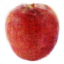
\includegraphics[width=0.33\columnwidth]{decoded-image-figure/densenet_nov11/Royal-Gala-Apple_decoded.png}}~
\subfigure[Brown Cap]{\label{subfig:brown-cap-natural}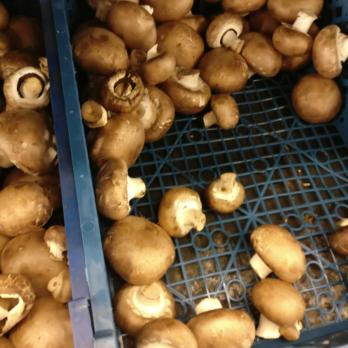
\includegraphics[width=0.33\columnwidth]{decoded-image-figure/Mushroom-Brown-Cap_027.jpg}}~
\subfigure[Decoded\,Brown\,Cap]{\label{subfig:brown-cap-decoded}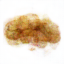
\includegraphics[width=0.33\columnwidth]{decoded-image-figure/densenet_nov11/Mushroom-Brown-Cap_decoded.png}}~
\subfigure[Oatgurt]{\label{subfig:oatgurt-natural}
\includegraphics[width=0.33\columnwidth]{decoded-image-figure/Oatly-Natural-Yoghurt_007.jpg}}~
\subfigure[Decoded Oatgurt]{\label{subfig:oatgurt-decoded}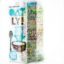
\includegraphics[width=0.33\columnwidth]{decoded-image-figure/densenet_nov11/Oatly-Natural-Yoghurt_decoded.png}}~ \\
\subfigure[Orange]{\label{subfig:orange-natural}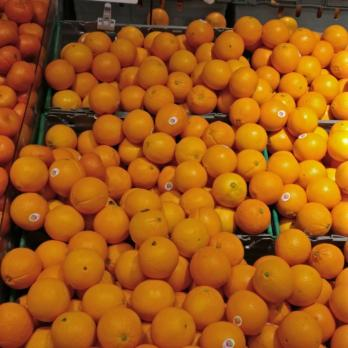
\includegraphics[width=0.33\columnwidth]{decoded-image-figure/Orange_056.jpg}}~
\subfigure[Decoded Orange]{\label{subfig:orange-decoded}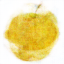
\includegraphics[width=0.33\columnwidth]{decoded-image-figure/densenet_nov11/Orange_decoded.png}}~
\subfigure[Onion]{\label{subfig:onion-natural}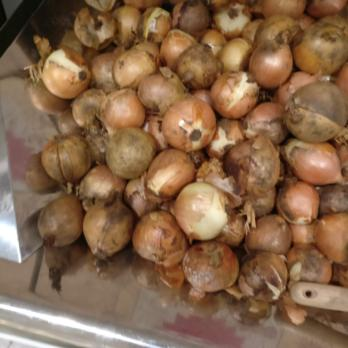
\includegraphics[width=0.33\columnwidth]{decoded-image-figure/Yellow-Onion_030.jpg}}~
\subfigure[Decoded Onion]{\label{subfig:onion-decoded}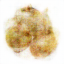
\includegraphics[width=0.33\columnwidth]{decoded-image-figure/densenet_nov11/Yellow-Onion_decoded.png}}~
\subfigure[Yogurt]{\label{subfig:yogurt-natural}
\includegraphics[width=0.33\columnwidth]{decoded-image-figure/Arla-Natural-Yoghurt_014.jpg}}~
\subfigure[Decoded Yogurt]{\label{subfig:yogurt-decoded}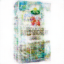
\includegraphics[width=0.33\columnwidth]{decoded-image-figure/densenet_nov11/Arla-Natural-Yoghurt_decoded.png}}~
\caption{ Examples of natural images in the test set that have been decoded into product iconic images by the iconic image decoder. This result is obtained with the fine-tuned DenseNet-169 features, which corresponds to VAE-CCA+SVM-ft in Table \ref{tab:results-fine-grained}. Subfigures (a), (c), (e), (g), (i) and (k) show the example input image from the test set, and Subfigures (b), (d), (f), (h), (j) and (l) show the decoded iconic image from the decoder $p_{\boldsymbol{\theta^{(2)}}}(\mathbf{y}\,|\,\mathbf{z})$ using VAE-CCA model as in Figure \ref{subfig:vae-cca}.} \label{fig:decoded-images}
\end{figure*}

The fine-grained classification results for all methods using an SVM as classifier are shown in Table \ref{tab:results-fine-grained}. We also provide coarse-grained classification results for some of the methods in Table \ref{tab:results-coarse-grained} to demonstrate the possibility of hierarchical evaluation that our labeling of the data provides (see Figure \ref{fig:examples}). The accuracies in the coarse-grained classification are naturally higher than the accuracies in the corresponding columns in Table \ref{tab:results-fine-grained}. Table \ref{tab:results-finetuned-cnn} shows fine-grained classification accuracies from a softmax classifier in the fine-tuned CNNs. We note that fine-tuning the networks gives consistently better results than training an SVM on off-the-shelf features (see Table \ref{tab:results-fine-grained}).

Fine-tuning the entire network results improves the classification performance consistently for each method in Table \ref{tab:results-fine-grained}. The performance is clearly enhanced for features extracted from fine-tuned VGG16 and DenseNet-169, which improves the classification accuracy by 10\% in most cases for SVM-ft, VAE+SVM-ft, and VAE-CCA+SVM-ft. For AlexNet and VGG16, we see that the performance drops when extracting the features from layer FC7 instead of FC6. The reason might be that the off-the-shelf features in FC7 are more difficult to transfer to other datasets since the weights are biased towards classifying objects in the ImageNet database. The performance drops also when we use fine-tuned features, which could be due to the small learning rate we use for the pretrained layers, such that the later layers are still ImageNet-specific. We might circumvent this drop by increasing the learning rate for the later pretrained layers and keeping the learning rate for earlier layers small.
 
The VAE-CCA model achieves mostly higher classification accuracies than the VAE model in both Table \ref{tab:results-fine-grained} and \ref{tab:results-coarse-grained}. This indicates that the latent representation separates the classes more distinctly than the VAE by jointly learning to reconstruct the extracted feature vectors and iconic images. However, further compressing the feature vectors with VAE and VAE-CCA will lower the classification accuracy compared to applying the feature vectors to a classifier directly. Since both VAE and VAE-CCA compresses the feature vectors into the latent representation, there is a risk of losing information about the natural images. We might receive better performance by increasing the dimension of the latent representation at the expense of speed in both training and classification.

In Figure \ref{fig:decoded-images}, we show results from the iconic image decoder $p_{\boldsymbol{\theta^{(2)}}}(\mathbf{y}\,|\,\mathbf{z})$ when translating natural images from the test set into iconic images with VAE-CCA and a fine-tuned DenseNet-169 as feature extractor. Such visualization can demonstrate the quality of the representation using the model, as well as enhancing the interpretability of the method. Using VAE-CCA in the proposed manner, we see that with challenging natural images, the model is still able to learn an effective representation which can be decoded to the correct iconic image. For example, some pears have been misplaced in the bin for Royal Gala apples in Figure \ref{subfig:royal-gala-natural}, but still the image decoder manages to decode a blurry red apple seen in Figure \ref{subfig:royal-gala-decoded}. In Figure \ref{subfig:orange-decoded}, a mix of an orange and an apple are decoded from a bin of oranges in Figure \ref{subfig:orange-natural}, which indicates these fruits are encoded close to each other in the learned latent space. Even if Figure \ref{subfig:oatgurt-natural} includes much of the background, the iconic image decoder is still able to reconstruct the iconic images accurately in Figure \ref{subfig:oatgurt-decoded}, which illustrates that the latent representation is able to explain away irrelevant information in the natural image and preserved the features of the oatgurt package. Thus, using VAE-CCA with iconic images as the second view not only advances the classification accuracy but also provides us with the means to understand the model.




\section{Conclusions}\label{paperC:sec:conclusions}

We propose learning the time to learn, i.e.,~in a real-world CL context, learning schedules of which tasks to replay at different times. %what previous tasks to replay at different times. 
To the best of our knowledge, we are the first to consider the time to learn in machine learning inspired by human learning techniques. 
We illustrate with MCTS how replay schedules can be learned and show that they can produce significantly improved results when comparing against methods without learned scheduling under the same memory budgets.
%We demonstrate with an example method that learned replay schedules produce significantly improved results under the same memory budget when comparing with the method without scheduling.
Furthermore, the dynamic behavior of the learned schedules showed similarities to human learning techniques, such as spaced repetition, by replaying previous tasks with varying time intervals.  
Finally, we showed that replay scheduling can be combined with any replay-based method as well as utilize the memory efficiently even when the memory size is smaller than the number of classes. %allows for utilizing the memory more efficiently compared to standard benchmarks replaying all memory samples in the tiny memory setting.
%Finally, we showed that replay scheduling allows for utilizing the memory more efficiently compared to standard benchmarks replaying all memory samples in the tiny memory setting.


In future work, we would like to explore choosing memory samples on an instance level as the current work selects samples on task level. 
This would need a policy learning method that scales to large action spaces which is a research challenge by itself. 
Also, using MCTS for learning replay scheduling policies can be inefficient, %our demonstrated method with MCTS can be inefficient, 
especially in CL settings, 
in terms of training time and since it needs to learn for each dataset and application separately. 
In future work, we will incorporate reinforcement learning methods that generalize and extend to learning general policies that can be directly applied to any new application and domain.
%In future work, we will incorporate reinforcement learning methods that generalize. We will therefore extend replay scheduling to learn general policies that can be directly applied to any new application and domain.



%\renewcommand*{\bibname}{References}
%\bibliographystyleA{unsrt}
%\bibliographyA{References/paperA_test}